% Sections 1 to 3.

\section{Introduction}\label{sec:intro}

A blockchain earns its existence only by serving a structural, growing and
badly served demand. Four currents converge in 2026 on the same point, and
no deployed chain occupies it: the nearest neighbors, reviewed in
Table~\ref{tab:neighbors}, each renounce at least two of its requirements.
The first is agent commerce. Coinbase revived HTTP status code 402 with the
x402 protocol, Stripe and Coinbase contest the machine-to-machine payment
rails, and four rival standards share the same territory. All of these rails
share three blind spots: they are denominated in stablecoins, they are fully
transparent, and they carry no portable trust. An agent pays on them;
nothing says whether it is reliable, for whom it acts, or who answers for
it. Yet a merchant cashing out an unknown agent, an accountant auditing a
fleet of agents, and a client delegating a budget all need the same thing:
to know who they are dealing with.

The second current is proof of humanity. Bots saturate the web to the point
that platform defense has become the separation of persons from programs.
The dominant answers are biometric: iris scans for one project, biometry
woven into consensus for another. Each accumulates the same debt, a body
measurement that is irreversible, centralized at collection even when the
proof is decentralized. Once an iris template is engraved somewhere, there
is no second chance; the perfect registry of future leaks is already
written. The third current is regulatory. MiCA and the FATF Travel Rule
keep sustained pressure on private coins, while Zcash demonstrates the
practicable path: a regulator who looks at its mechanism understands it,
shielded pools, viewing keys, explicit disclosure. Readability, not
transparency, is the acceptance criterion. The fourth current is
instantaneity. A counter payment must become irreversible in seconds; the
existing private chains require tens of seconds to minutes of real
finality.

\begin{table}[htbp]
\centering
\small
\caption{The four demands of 2026 and the empty square at the center.}
\label{tab:demands}
\begin{tabularx}{\textwidth}{@{}L{4.1cm}YY@{}}
\toprule
Demand in 2026 & Dominant offer & Blind spot left open \\
\midrule
Agent payments (x402, MPP, ACP, AP2) & HTTP rails on transparent stablecoins &
portable trust, privacy, a designated answerable party: none \\
Proof of humanity & biometrics (iris, face, veins) &
non-biometric personhood, with no body registry \\
Sustainable privacy (MiCA, Travel Rule) & Zcash: selective disclosure; Monero: opacity &
native privacy with provable compliance \\
Quasi-instant private payment & Kaspa (fast, transparent); Monero (private, slow) &
fast, private, finalized in seconds, on egalitarian hardware \\
\bottomrule
\end{tabularx}
\end{table}

\begin{table}[htbp]
\centering
\small
\caption{The neighbors of the square, and what each renounces. The
reference here is honest: rings and fast DAG ordering are inherited arts,
not inventions of this paper.}
\label{tab:neighbors}
\begin{tabularx}{\textwidth}{@{}L{3.2cm}Y Y@{}}
\toprule
Chain & Closest strength & What it renounces of the five properties \\
\midrule
Monero, NERVA & the reference of private payment & speed (minutes of finality), agent identity, disclosure levels \\
Zcash (Orchard) & readable selective disclosure & egalitarian CPU mining (Equihash ASIC territory), agent identity, speed \\
Kaspa & fast DAG ordering at scale & privacy entirely, disclosure, reputation \\
Xelis & encrypted amounts on a DAG & ring anonymity (no decoys), reputation, CPU-only mining \\
Penumbra, Namada & shielded multi-asset, ZK disclosure & CPU mining, egalitarian hardware, reputation as consensus \\
Aztec, Aleo & private general computation & every proof circuit is maximal technique and maximal audit surface; CPU mining \\
ANTUMBRA & the five properties together & general masked contracts, honestly deferred (Section~\ref{sec:contracts}) \\
\bottomrule
\end{tabularx}
\end{table}

The center of Table~\ref{tab:demands} is empty, and not for technical
reasons. It is empty because each ecosystem optimized a single dimension:
agent rails optimized throughput, biometrics optimized anti-sybil, Zcash
optimized regulatory legitimacy, Kaspa optimized speed. None of them treats
trust, meaning who acts, since when, answerable up to which human, as a
primitive of the protocol. The network that installs trust there must
combine five properties usually considered incompatible: speed, privacy by
default, provable disclosure, processor egalitarianism, and a reputation
that capital cannot fabricate. The thesis of this paper is that these
properties reinforce one another as soon as one of them, reputation
anchored in time, is treated as the foundation.

The monetary and consensus numbers that recur throughout this document are
gathered here for reference. Each is justified in the section indicated.

\begin{table}[htbp]
\centering
\small
\caption{Reference magnitudes of the network.}
\label{tab:magnitudes}
\begin{tabularx}{\textwidth}{@{}L{3.6cm}L{4.4cm}Y@{}}
\toprule
Quantity & Value & Meaning \\
\midrule
Monetary cap & 16,180,339 ATU & the golden ratio scaled by ten million; the same proportion already drives RandomX \\
Emission & 34 eclipses of 4 years & each eclipse emits 61.8\,\% of the previous one; the cap is reached exactly at year 136 \\
Blocks & 2 seconds & near-immediate inclusion; the DAG absorbs parallel blocks \\
Economic finality & under 6 seconds & checkpoints signed by the Ring, quorum of 37 out of 55 seats \\
Privacy & private by default & rings of sixteen, committed amounts, one-time addresses, Tor by default \\
Disclosure & selective, three levels & per transaction, per bounded auditor, per compliance proof \\
Reputation & Kleos, 0 to 100 & Deed 40, Echo 30, Tenure 30; non-transferable, corroded by time \\
Premine & 0\,\% & everything is mined or governed; nobody starts with an advantage \\
\bottomrule
\end{tabularx}
\end{table}

\section{Design Overview}\label{sec:overview}

ANTUMBRA separates cleanly what most chains pile up: settlement, finality,
identity and disclosure. The settlement layer, at the bottom, is a
CPU-mined BlockDAG that orders parallel blocks every two seconds and
carries private-by-default transactions: this is the Veil. The finality
layer, the Ring, is a committee of fifty-five high-reputation identities
that sign checkpoints every four seconds and make any payment irreversible
in under six seconds. The identity layer distinguishes humans, the Embers,
from agents, the Ciphers, with their admission and accountability rules.
The reputation layer, Kleos, feeds the Ring, locks sponsorships and weights
peer testimony. Around the whole, the Lumen, selective disclosure, forms
the ring of light that gives the network its name: a shadow faithfully
kept, proofs on demand.

\begin{figure}[htbp]
\centering
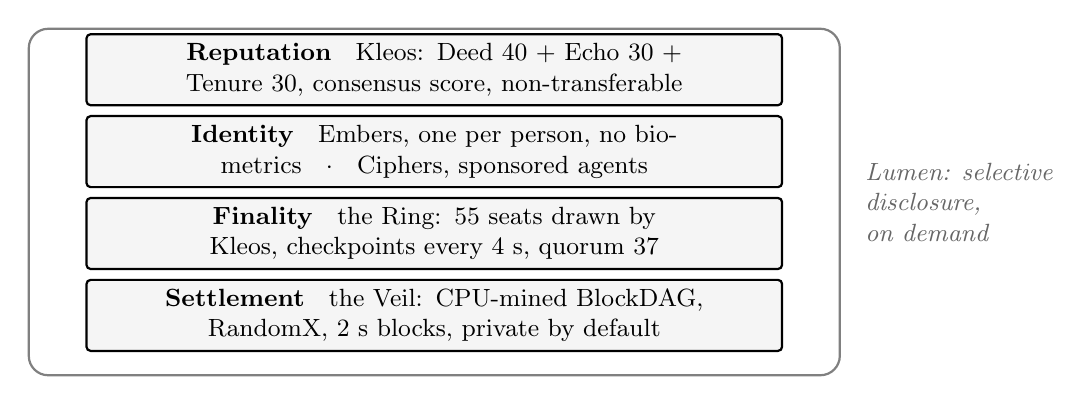
\begin{tikzpicture}[
  layer/.style={draw=black, thick, rounded corners=1.5pt, text width=8.6cm,
                minimum height=0.82cm, align=center, font=\small, fill=black!4},
]
  % Lumen enclosure
  \draw[rounded corners=7pt, thick, black!50]
        (-5.15,-0.78) rectangle (5.15,3.62);
  \node[anchor=west, font=\small\itshape, text=black!60, align=left]
        at (5.35,1.42) {Lumen: selective\\disclosure,\\on demand};
  % the four layers, top to bottom
  \node[layer] (rep) at (0,3.1)
    {\textbf{Reputation} \; Kleos: Deed 40 + Echo 30 + Tenure 30, consensus score, non-transferable};
  \node[layer] (ide) at (0,2.06)
    {\textbf{Identity} \; Embers, one per person, no biometrics \; $\cdot$ \; Ciphers, sponsored agents};
  \node[layer] (fin) at (0,1.02)
    {\textbf{Finality} \; the Ring: 55 seats drawn by Kleos, checkpoints every 4 s, quorum 37};
  \node[layer] (set) at (-0.0,-0.02)
    {\textbf{Settlement} \; the Veil: CPU-mined BlockDAG, RandomX, 2 s blocks, private by default};
\end{tikzpicture}
\caption{The four layers of ANTUMBRA inside the Lumen, the selective
disclosure ring. Each layer depends only on the layers below it.}
\label{fig:arch}
\end{figure}

The nomenclature is stable across the document; each name designates one
precise part and only one. The reader may return to Table~\ref{tab:naming}
at any time. The internal names are working codenames, chosen to keep the
document readable; they may be adapted at implementation time. Only
ANTUMBRA and its ticker ATU are proposed as a definitive commitment,
verified free of collision on the blockchain and crypto namespace on
September 6, 2026. One layer of Table~\ref{tab:naming} sits above the
others and outside the stack discipline: the Corona,
Section~\ref{sec:corona}, machine governance that reads every layer and
modifies none of them without the human chambers.

\begin{table}[htbp]
\centering
\small
\caption{Reference nomenclature.}
\label{tab:naming}
\begin{tabularx}{\textwidth}{@{}L{2.2cm}L{3.4cm}Y@{}}
\toprule
Name & Nature & Role in one sentence \\
\midrule
ANTUMBRA & the network & private settlement BlockDAG, CPU-mined \\
ATU & the currency & 16,180,339 units, divisible by $10^{8}$ \\
the Veil & privacy & rings of sixteen, committed amounts, one-time addresses, Tor by default \\
the Lumen & disclosure & hierarchical viewing keys and compliance proofs, on demand \\
the Ember & human identity & one per person, non-biometric, one vote in governance \\
the Cipher & agent identity & sponsored by an Ember, with a revocable spending perimeter \\
Kleos & reputation & three-layer score, consensus, non-transferable, non-purchasable \\
the Ring & finality committee & 55 high-reputation seats, checkpoints every 4 seconds \\
RAF & finality mechanism & Reputation-Anchored Finality \\
the Corona & machine governance & AI senators that propose, red-team and implement changes under human veto (Section~\ref{sec:corona}) \\
the Vault & deployment custody & threshold signature of 9 hardware fragments, 7 needed, no whole key anywhere \\
era & protocol time & six months; the unit of reputation, rotation and decay \\
eclipse & emission time & four years, eight eras; 34 eclipses lead to the cap at year 136 \\
Mandate & money contract & an output whose release obeys a predicate declared at creation \\
the Machine & logic contract & deterministic virtual machine on public state only, after genesis \\
\bottomrule
\end{tabularx}
\end{table}

Two principles govern the assembly. First, each layer depends only on the
layers below it: settlement ignores reputation, finality reads Kleos but
never writes it, identity builds on both without modifying either. That
stacking discipline is what keeps every part auditable in isolation and
replaceable without rewriting the rest. Second, the value loop: reputation
protects finality, finality makes payments instant, instant payments serve
agents and merchants, and their honorable behavior enriches reputation.
The network is designed so that its security and its utility feed each
other instead of taxing each other.

\section{The Settlement Layer: a CPU-Mined BlockDAG}\label{sec:settlement}

The first wager is egalitarian. RandomX, the algorithm designed so that one
ordinary computer is one vote, produces blocks that no specialized machine
produces better at equal cost: no dedicated circuit, no farm of graphics
cards. Miners run it in fast mode, 2,080 MiB of memory; verifying nodes
may run light mode, 256 MiB of cache and no dataset, a size its author
chose deliberately so that specialized hardware gains nothing by verifying:
the light-mode memory-time product was sized to close exactly that door.
Emission and block production stay within reach of anyone who owns
a laptop, the ethos of NERVA carried to its conclusion. The constant
\texttt{0x9E3779B9}, the integer truncation of the golden ratio in binary
arithmetic, already drives the generation of RandomX superscalar programs;
the same proportion that will distribute the currency already works inside
the engine that will mine it, a mnemonic accident the paper claims as
identity, not as argument.

The second wager is structural. A linear chain must choose between short
blocks, which multiply orphans, and long blocks, which slow confirmation;
a DAG orders parallel blocks instead of rejecting them. At a two-second
cadence, a linear proof-of-work network would lose an unsustainable share
of its blocks; a fast-converging DAG integrates them into its partial
order and accumulates the work of all of them. Speed stops being a
trade-off against egalitarianism: it becomes its product. The ordering
layer belongs to the GHOSTDAG family, whose public literature and existing
implementations provide the operational definitions of convergence and
anticone.

\begin{table}[htbp]
\centering
\small
\caption{Parameters of the settlement layer.}
\label{tab:settlement}
\begin{tabularx}{\textwidth}{@{}L{4.0cm}L{4.6cm}Y@{}}
\toprule
Parameter & Retained value & Justification \\
\midrule
Mining algorithm & RandomX: fast mode 2,080 MiB, light mode 256 MiB & proven by years of attack; the light-mode cache is sized so verification resists specialization \\
Block cadence & 2 seconds & near-immediate inclusion; the DAG absorbs the orphan rate \\
Block ordering & GHOSTDAG-family coloring, cluster parameter $k = 8$ & security grows with block volume, not only depth; $k$ is calibrated for the two-second cadence \\
Flow anonymity & ring of 16, masked amounts & equals the strongest ring deployed in the lineage (Monero since 2022); a floor to raise, not a ceiling \\
Signature scheme & MLSAG over Ed25519, Keccak-256 & the lineage construction, implemented and cross-validated; CLSAG is the post-audit upgrade candidate \\
Transport network & Dandelion++, Tor for transaction injection & IP-address analysis is the number one practical flaw of private chains \\
Finality & Ring checkpoints (Section~\ref{sec:ring}) & economic irreversibility in under 6 seconds \\
Target throughput & 100 tx/s sustained, 300 tx/s burst, on the reference node & an engineering budget with a measured exit criterion (Table~\ref{tab:capacity}) \\
Storage & pruned DAG, decoy pool retained forever & the nullifier set and output keys are consensus data; the growth budget is stated in Table~\ref{tab:capacity} \\
\bottomrule
\end{tabularx}
\end{table}

Pruning deserves its own paragraph, because it conditions the entire social
contract, and in a ring chain it is not free: spent outputs remain decoys
for everyone else's privacy, so the output keys, their commitments and the
nullifier set are consensus data forever, roughly ninety-six bytes per
output. What prunes is the rest: the ring signatures, the range proofs and
the transaction bodies beyond the recent window, which no later
verification re-reads. A network whose nodes required a disk bay would
exclude exactly the participants it claims to serve; the growth budget of
Table~\ref{tab:capacity} keeps that promise measurable. Dandelion++ stem
propagation and Tor transport close the door on IP-address analysis, which
remains the great practical weakness of badly configured private networks:
transactional privacy is nothing if the network observer knows who emitted
what. One precision, because latency and a DAG interact: transactions are
injected through Tor, but blocks relay node to node over the peer network
with mandatory encryption, so the stem anonymity of a payment never slows
the ordering of blocks that carry it, and the cluster parameter $k$ is
calibrated against measured propagation at the two-second cadence, an exit
criterion of the prototype phase, not an assumption.

\subsection{The DAG contract, stated precisely}

A specification that grafts rings onto a DAG must say exactly where the
seams are. The rules, frozen here and implemented in the reference node:
\begin{enumerate}[leftmargin=1.7em, itemsep=3pt, topsep=4pt]
\item \textbf{Ordering.} The coloring is GHOSTDAG-family with cluster
parameter $k = 8$: a block is blue when its anticone in the selected
parent's past is at most $k$; the blue score accumulates, the selected
parent maximizes it, and the consensus order is the depth-first walk of the
selected-parent chain absorbing blue blocks, then the remaining red blocks
in insertion order. Deterministic in the accepted set alone.
\item \textbf{Validity resolves in consensus order, not arrival order.} A
double spend published in parallel blocks is resolved by the order: the
first occurrence in consensus order spends the output, every later
occurrence is rejected at ordering time. The nullifier registry, the set of
published key images, is keyed by this order, so two conflicting
transactions in one anticone have exactly one winner, decided by a rule
every node recomputes identically.
\item \textbf{Decoys are drawn from the ordered past.} A wallet samples
decoys only from outputs already ordered by the DAG, never from the
anticone: an unordered output may yet be a parallel spend, and a decoy that
could become invalid is a decoy that betrays the real signer. Age brackets
follow the real spending distribution, the lineage's known discipline.
\item \textbf{Scanning.} Every output carries a one-byte view tag derived
from the shared secret: a wallet skips the full elliptic-curve derivation
for the outputs the tag does not match, so scanning stays linear and cheap
at any block cadence.
\item \textbf{Pruning.} Output keys, commitments, encrypted amounts and
nullifiers are retained forever; signatures, range proofs and bodies prune
after the verification window. Archival nodes keep everything by choice,
never by obligation.
\end{enumerate}

\subsection{The capacity budget, stated as numbers}

A private network that claims a throughput must show its arithmetic,
because privacy is precisely what makes verification expensive. The
reference node is a 2020-class desktop, four cores and eight gibibytes.
One standard transfer, two inputs and two outputs at ring sixteen,
verifies in about ten milliseconds of single-core work, dominated by the
MLSAG chains and the aggregated range proof; four cores therefore clear on
the order of four hundred transactions per second of pure verification,
before memory and bandwidth contend. The budget below is the honest form
of the claim: targets are what the exit criteria measure on the prototype
network, and the sustained expectation of a payment network of this size
is five to twenty transactions per second for the first years; the hundred
is headroom against spikes, not a promise of volume.

\begin{table}[htbp]
\centering
\small
\caption{The capacity budget of the reference node (4 cores, 8 GiB), and
what each target commits to.}
\label{tab:capacity}
\begin{tabularx}{\textwidth}{@{}L{3.1cm}Y Y@{}}
\toprule
Resource & Budget & Consequence \\
\midrule
Verification & $\sim$10 ms per tx, single core; 4 cores in parallel & the phase-1 exit criterion: 100 tx/s sustained for 24 h on the reference node \\
Bandwidth & $\sim$1.5 kB per tx, $\sim$1.5 Mbit/s sustained; 4.5 Mbit/s at burst & fits any residential connection; measured on the prototype, not asserted \\
Decoy pool growth & $\sim$192 B per tx: 56 GiB per year at 10 tx/s, 564 GiB if 100 tx/s were held for a year & the ceiling is burst capacity, not a promise; at the sustained expectation a one-terabyte disk holds the pool for a decade \\
Pruned node body & signatures and proofs beyond the window pruned & the 1 TiB disk also holds the recent bodies with ample margin \\
Burst ceiling & 300 tx/s for minutes on 8-core hardware & validated on the test network before phase five, or the sustained target drops \\
\bottomrule
\end{tabularx}
\end{table}

One honest word to close the section: grafting a fast-converging DAG onto
a CryptoNote base is a real engineering challenge, work of substance and
not a configuration flag. The roadmap (Section~\ref{sec:roadmap}) treats
it as the first technical risk of the project, with an isolated prototype
and a dedicated audit before any main network. The rules above make the
seam precise: cluster parameter, order resolution, decoy sampling,
scanning and pruning are stated, implemented and cross-validated, the
literature is public and solid, and none of the primitives used is exotic:
the risk is a degree of difficulty, not a degree of uncertainty.
